\documentclass[12pt,letterpaper, oneside]
{article}
\usepackage[utf8]{inputenc}
% \usepackage[T1]{frontenc}
\usepackage{graphicx,subcaption}
\usepackage{wrapfig,booktabs}
\graphicspath{ {../img/} }

\usepackage{floatrow}
	\DeclareFloatFont{Small}{\fontsize{9}{11}\sffamily}
	\floatsetup{font = Small}

\usepackage{geometry}
	\geometry{
		a4paper,
		total={170mm,257mm},
		left=20mm,
		top=20mm
	}

% \usepackage{caption}
	% \captionsetup{belowskip=-20pt}

\usepackage{array,multirow,float}
\usepackage[affil-it]{authblk} 
\renewcommand\Affilfont{\fontsize{9}{10.8}\itshape}

\title{Mining Toronto Fire Services Incident Data}
\author{Geoffrey Clark}
\affil{Prepared for Dr. Ceni Babaoglu
\\ CKME136: Data Analytics Capstone Course 
\\ Data Science Lab, Ryerson University}

\begin{document}

\maketitle
\vspace{-1cm}
\begin{abstract}
The goal of this project was to explore the viability of 'classical' machine learning algorithms on a fire incident data set. An open source data set on Toronto Fire Services Incidents was obtained, cleaned and the subject of some exploratory analysis. A binary class attribute was assigned to each incident based on post-incident features such as damage and number of responding units. Three machine learning algorithms—Logistic Regression, Naive Bayes and Random Forest—were then used to predict the class attribute using features whose values would be known at the time of incident call. The results are presented and discussed.
\end{abstract}

\tableofcontents 

% \section{Overview}
% \begin{itemize}
% 	\item Introduction
% 	\item Literature Review
% 	\item Dataset
% 	\item Approach
% 	\item Exploratory Analysis
% 	\item Modeling
% 	\item Results
% 	\item Conclusions
% \end{itemize}

\section{Introduction}

Emergency Services in general, and the Fire Brigade in particular, are in constant demand and often in situations where they find themselves at risk. Any additional information that can be provided to the Fire Services at the time of an incident may prove invaluable in improving performance and success. Computer Aided Dispatch systems, already in use (Bebee, D. 2012), provide a huge opportunity: both in their logging of data and their integration within the emergency services systems. An effective machine learning model, appropriately trained, may be able to provide first responders with insights about the incidents that they are responding to before they arrive and thus help reduce cost, time and risk (Asgary, A.,\& Sadeghi-Naini, A. 2012). This project explores the viability of such a model and compares three well known machine learning algorithms: Logistic Regression, Naive Bayes, and Random Forest. 

\section{Literature Review}
There is a wide array of fire incident research and evidence of agreement to its inherent value (Sekizawa, A., 2012). Research exists on training Neural Networks to predict fire incident characteristics such as risk (A., Naini, AS., \& Levy, J. 2012), number of firefighters responding (Asgary, A., \& Sadeghi-Naini, A., 2013), loss and no-loss fire incidents (Asgary, A., Sadeghi-Naini, A., \& Kong, A., 2009), and critical incidents (Asgary, A., Sadeghi-Naini, A., \& Levy, J., 2009). These approaches were all relatively successful in their goals, however, complex models such as Deep Learning and Artificial Neural Networks often have associated costs such as additional complexity and may be more difficult to interpret as a result (G. Casella, S. Fienberg, I. Olkin, 2013, p. 25). It is prudent to explore traditional methods before adopting a more complex solution while maintaining a constant awareness of the trade-offs and costs associated with the more complex solution.

% \begin{wrapfigure}[28]{l}{0.5\textwidth}
% \begin{tabular}{ p{0.25\textwidth} p{0.25\textwidth} }
% \begin{wraptable}{l}{5.5cm}
\begin{wraptable}[21]{l}{0.5\textwidth}
\vspace{-1cm}
% \begin{table}
% \small

% \begin{tabular}{ll}\\\toprule
\begin{tabular}{ p{0.40\textwidth} p{0.50\textwidth} }
\\\toprule
Feature & Description \\\midrule 
EVENT\_TYPE & Type of event: Medical, fire, etc \\ \midrule
INCIDENT\_DATE & Date of initial call \\ \midrule
RESPONDING\_UNITS & Number of units who responded (total) \\ \midrule
RESPONSE\_TYPE & Type of response: Rescue, medical, etc \\ \midrule
PROPERTY\_TYPE & Type of property \\ \midrule
ALARM\_TO\_FD & Source of call \\ \midrule
EST\_KM & Estimated Distance to Incident \\ \midrule
INITIAL\_UNIT\_\newline PERSONNEL & Number of personnel responding on first apparatus \\ \midrule
EST\_LOSS & Estimated loss due to incident \\ \midrule
EST\_VALUE\_AT\_RISK & Estimated value at risk \\ \midrule
FF\_INJURIES & Firefighter Injuries \\ \midrule
FF\_FATALITIES & Firefighter Fatalities \\ \midrule
CIVILIAN\_INJURIES & Civilian Injuries \\ \midrule
CIVILIAN\_FATALITIES & Civilian Fatalities \\ \midrule
RESCUES & Number of rescues \\ \midrule
OFM\_INVESTIGATIONS\_\newline CONTACTED & Office of Fire Marshall Investigations unit contacted \\ \midrule
INCIDENT\_DAY, MONTH, HOUR, ... & Extracted from INCIDENT\_DATE \\ \bottomrule
\vspace{-4cm}
\caption{
	% \vspace{-4cm}
	Features used in this project.}\label{tab:1}

\end{tabular}
\end{wraptable}
% \end{table}
% \end{wrapfigure}

Fire services incident data has been the subject of other types of research also, including spacial and temporal analysis in both Toronto, Canada (Asgary, A., Ghaffari, A., Levy, J., 2009) and Ankara, Turkey (Ceyhan, E., Ertŭgay, K., \& Düzgün, Ş., 2013). International scope is not limited to Japan, Canada and Turkey, however, as research has been published on the implementation of fire incident reporting systems and their value in the United States as well (Bergen, G., Frattaroli, S., Ballesteros M.F., Ta, V.M., Beach, C., \& Gielen, A.C., 2008).

\section{Dataset}

The dataset used in this project was both a great resource and large challenge. Retrieved in May, 2018, from the Toronto Open Data Catalogue the dataset contains 720,370 records of Toronto Fire Services Incidents from the years 2011 through 2016. Up to 100 features are provided from multiple sources including the Computer Aided Dispatch System and Office of the Fire Marshall Incident Reports. 

% \includegraphics[scale=0.5]{Incidents_by_year}
\begin{wrapfigure}{R}{0.40\textwidth}
	% \vspace{-50pt}
	\centering
	\includegraphics[width=\textwidth]{Incidents_by_year}
	\caption{Yearly breakdown of incident quantities
		\label{fig:yearly}
	}
	
\end{wrapfigure} 

Each observation in the data set corresponds to an incident such as fire, medical call, or police assist and has a corresponding unique identifier. Some features, such as incident number, event type and alarm source appear to have been available at the time of incident call and are most likely inputted by the Computer Aided Dispatch (CAD) system. This characteristic of being inputted automatically has led to these features being relatively reliable and complete compared to others in the dataset. 

Also present in the dataset are features that contain values which would be entered, most likely manually, following an incident and include such features as estimated damage, number of firefighter and civilian injuries and casualties, number of rescues, and if the Office of the Fire Marshall (OFM) Investigations Department was contacted. The features used in the analysis and modeling sections of this project were chosen largely for their completeness and time of input: before or after the incident. Some features, such as highest alarm level reached and which fire department station dispatched, were dropped due to lack of availability or obfuscated values. 

The breakdown of number of incidents by year in Figure~\ref{fig:yearly} reveals a relatively constant trend of incidents with a slightly higher amount in the first year of the dataset, 2011. 

\section{Approach}
\begin{wrapfigure}[22]{l}{0.40\textwidth}
	\centering
	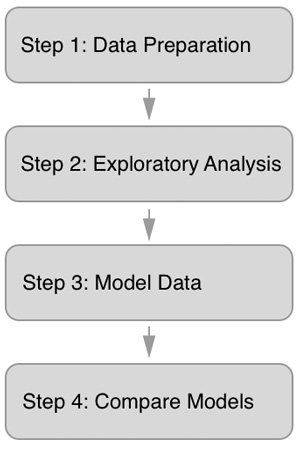
\includegraphics[width=\textwidth]{block-diagram}
	\caption{
		A block diagram of this project approach.
		\label{fig:blocks}
	}
\end{wrapfigure}

This project's approach was to first import, clean and prepare the dataset, secondly perform an exploratory analysis, thirdly to train \& test a predictive model on a dependent variable of choice, and finally to evaluate the models performance. A graphical outline is provided in Figure~\ref{fig:blocks}.


\medskip\noindent\textbf{Step 1: Data Preparation}
\\*Published as separate XML files the data was initially in a difficult structure for analysis and thus converted into tabular structure with each row representing an observation (incident) and each column representing an attribute (feature). Following conversion each feature was inspected quantitatively, for NA values, summary statistics, and qualitatively, for source, description, and time of input relative to the incident. 

\medskip\noindent\textbf{Step 2: Exploratory Analysis}
\\*Following the conversion and initial preparation stage an exploratory analysis was conducted where features and relationships were examined in more detail. The primary concern of this step was to improve understanding of the data. Univariate, bivariate and multivariate relationships among features were examined. It was during this exploratory analysis that features were examined for their suspected relevance in defining or predicting the class variable. 

\medskip\noindent\textbf{Step 3: Model Data}
\\*Following the initial analysis three models, Logistic Regression, Naive Bayes and Random Forest, were used to predict the class attribute. The models were used to classify the class attribute on a subset containing only fire incidents in order to reduce a class imbalance. During this process the models were trained on 10 randomly selected training sets and then tested on the corresponding test sets. This procedure, similar to k-fold cross validation, was to determine the presence of high-variance (overfitting) of the models. 

\medskip\noindent\textbf{Step 4: Compare Models}
\\*After training and running the models the results are accumulated and compared using four metrics: Accuracy, Recall, Precision and F\textsubscript{1}-Score. F\textsubscript{1}-Score is weighted heavier than accuracy due to the former's tendency to be low in the absence of any True Positives, a situation that can result in the presence of a strong class imbalance.

\section{Exploratory Analysis}

\begin{wrapfigure}[28]{l}{0.50\textwidth}
	\centering
	\begin{subfigure}[b]{\textwidth}
		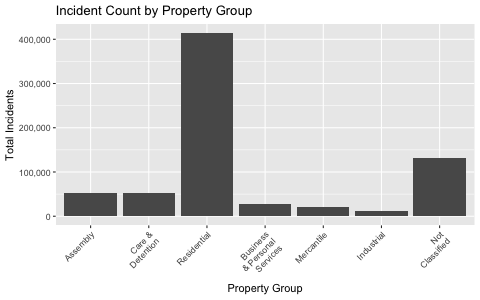
\includegraphics[width=\textwidth]{incident-count-by-property-group}
		\caption{
			Total incident count for each property type (grouped for similarity): Residential accounts for over 50\% of all incidents
			\label{fig:cnt-prop}
		}
	\end{subfigure}
	\begin{subfigure}[b]{\textwidth}
		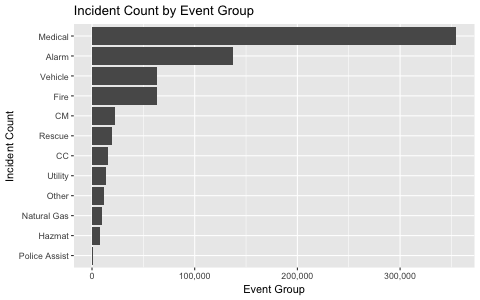
\includegraphics[width=\textwidth]{incident_count_by_event_group}
		\caption{
			Total incident account for each event type (grouped for similarity): Medical accounts for nearly 50\% of all incidents.
			\label{fig:cnt-event}
		}
	\end{subfigure}
	\caption{Total incident counts for property \& event groupings.
		\label{fig:prop-event}
	}
\end{wrapfigure}

\subsection{Event \& Property Type}
Considering every incident an event that happens at some type of property facilitates the types of breakdown shown in Figure~\ref{fig:prop-event}; total incidents by property group and event group, respectively. Both groups have been combined by combining many similar types of levels into one; otherwise the features themselves would have far too many features (115 in the case of event type). It is clear from these figures that the most numerously occurring property type is by far Residential while Medical events occur for nearly half of all incidents (approximately 350,000/720,000). 
Regarding the source of data, event type is likely available before the incident as the feature \textsf{EVENT\_TYPE\_CD} (Event Type Call Dispatched) contains event type information that is dispatched before the arrival of first responders. Property type, however, is sourced from the OFM Standard Incident Codes List and is thus likely inputted following an event.

\subsection{Alarm to Fire Department, Event Group}
The Alarm to Fire Department feature, \textsf{ALARM\_TO\_FD}, describes the source of incident report. \textsf{EVENT\_GROUP} is a \\*grouping of different types of event. The features are related in the sense that \textsf{ALARM\_TO\_FD} is the input source (911, Police, etc) whereas \textsf{EVENT\_GROUP} describes the type of incident the call turned out to be. Perhaps a reasonable expectation would be that certain types of calls correspond to certain types of events.

\begin{wrapfigure}{r}{0.50\textwidth}
	
	\centering
		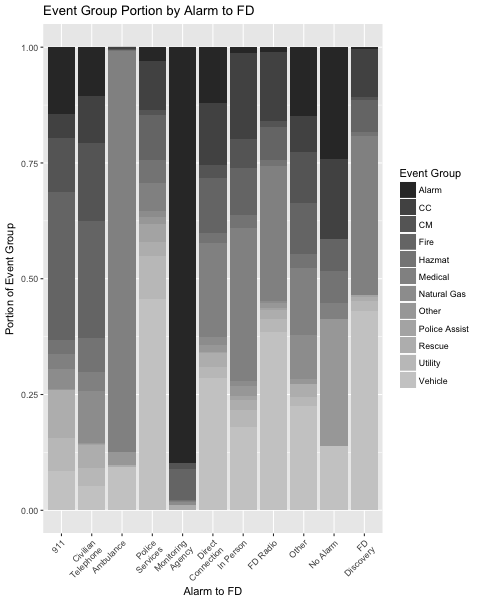
\includegraphics[width=\textwidth]{event-group-portion_vs_alarm-to-fd-BW}
		\caption{The portion of Event Types (grouped for similarity) for each call source (Alarm to FD).
			\label{fig:event-alarm}
		}
	% \rule{12cm, 8cm}
\end{wrapfigure} 

The visual in Figure~\ref{fig:event-alarm} displays the portion of Event Type Group by Call Source (Alarm to Fire Department) and suggests that the source of call will impact which type of call is received. For example, if an incident is reported by a Monitoring Agency there is greater than a 75\% chance that the Event Type will be an Alarm.


\subsection{Temporal Feature Analysis}
This dataset includes multiple temporal features including Incident and Dispatch Date as well as corresponding times for when the call was first received, when first responders initially arrived on the scene, and when the incident was controlled. 

A breakdown of incident quantities by hour and day is provided in Figure~\ref{fig:cox}. In general, the trend of number of incident calls received increases from a low around 4 am where they begin to increase until the max which occurs at approximately 6pm. After 6pm the quantity of incidents per hour tends to decrease again until 4 am. This cycle is pretty standard for Monday through Thursday, however, Friday through Sunday show increased relative call volumes in the evening when compared to weekdays. There is also a noticeable increase in call volumes early Sunday morning where activity from Saturday night would be carried over. 

\begin{figure}[h]
	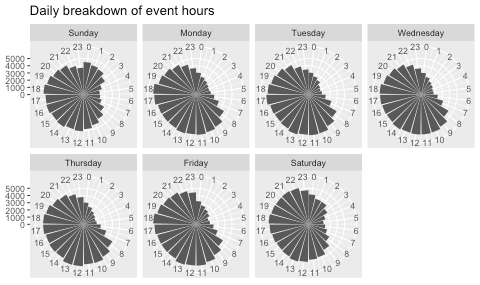
\includegraphics[scale=0.6]{daily-hourly-coxwell-crop}
	\caption{Incident counts grouped by hour and day. There is increased incident quantities on Weekend evenings (Friday, Saturday, Sunday morning) versus the weekdays. 
	\label{fig:cox}}
\end{figure}

\subsection{Association Rules}

Association rules were run on all observations of the following features: \textsf{EVENT\_GROUP, ALARM\_TO\_FD, RESPONSE\_GROUP, PROPERTY\_GROUP, MONTH, DAY, HOUR, EVENT\_TYPE\_CD}. No rules were found with the three temporal features (\textsf{MONTH, DAY, HOUR}), however, other interesting patterns were discovered. Five such rules are presented in Table~\ref{tab:arules} with corresponding summaries below. \\*

\begin{table}[h]
	\hspace*{-0.3cm}
	\begin{tabular}{p{0.01\textwidth} p{0.5\textwidth} p{0.1\textwidth} p{0.1\textwidth} p{0.1\textwidth} p{0.1\textwidth}} \toprule
		\# & Rules & Support & Confidence & Lift & Count \\ \midrule
		1 & \{Event group = Alarm, Property Group = Residential\} $\Rightarrow$ \{Alarm to Fire Department = From Monitoring Agency\} & 0.1019 & 0.8294 & 4.7289 & 73398 \\ \midrule 
		2 & \{Event group = Alarm\} $\Rightarrow$ \{Response Group = False Fire Calls\} & 0.1564 & 0.8178 & 3.9498 & 112659 \\ \midrule
		3 & \{Event group = Alarm, Alarm to Fire Department = From Monitoring Agency\} $\Rightarrow$ \{Response Group = False Fire Calls\} & 0.1282 & 0.8145 & 3.9340 & 92345 \\ \midrule
		4 & \{Response group = Medical/resuscitator call, Event type call as dispatched = Medical\} $\Rightarrow$ \{Event group = Medical\} & 0.1920 & 1.0000 & 2.0307 & 138287 \\ \midrule
		5 & \{Alarm to Fire Department = From Ambulance, Event type call as dispatched = Medical\} & 0.2123 & 1.0000 & 2.0307 & 152920 \\
		\caption{
			Association Rules with Corresponding Support, Confidence, Lift and Total Count. 
			\label{tab:arules}
		} 


	\end{tabular}
\end{table}


\begin{enumerate}

\item \textsf{\{Event group = Alarm, Property Group = Residential\} $\Rightarrow$ \{Alarm to Fire Department = From Monitoring Agency\}}

This rule describes incidents where the Fire Services responded to Residential Alarms. Of these alarms, 82\% (confidence) were received from a monitoring agency. 
\item \textsf{\{Event group = Alarm\} $\Rightarrow$ \{Response Group = False Fire Calls\}}

This simple statistic, also with high lift (3.9), shows that 81\% of the alarms that the fire services respond to are false fire calls. This is an incredibly high percentage and represents approximately 15\% of all incidents in this dataset. 
\item \textsf{\{Event group = Alarm, Alarm to Fire Department = From Monitoring Agency\} $\Rightarrow$ \{Response Group = False Fire Calls\}}

This rule elaborates on rule \#2 by showing that a high percentage (approximately 82\%) of aforementioned false alarm calls are received from a monitoring agency.
\item \textsf{\{Response group = Medical/resuscitator call, Event type call as dispatched = Medical\} $\Rightarrow$ \{Event group = Medical\}}

This rule perhaps seems obvious but is worth noting: with a confidence of 100\%, all incidents responded to as medical calls, which were dispatched as medical calls, ended up being classified as medical calls. This data set has a high proportion of medical calls. Note that only 138,000 of the some 350,000 medical incidents in this data set fit that pattern. This suggests that there is some variability among these features of medical calls.
\item \textsf{\{Alarm to Fire Department = From Ambulance, Event type call as dispatched = Medical\} $\Rightarrow$ \{Event group = Medical\}}

As with rule \#4 this is perhaps a sanity check (despite a lift value of 2) and may seem as expected: Every incident received from an Ambulance is dispatched as Medical with an event type categorized as Medical. This stipulates that ambulances make no other calls to the fire services besides medical calls. 
\end{enumerate}

\section{Modeling}
\subsection{Model Selection}
To proceed with modeling fire risk was chosen as a dependent variable and risk was first categorized according to criteria provided in prior research and secondly by extending the classification thresholds in order to reduce a significant class imbalance. After assigning the dependent attributes three classifiers were run to predict the class variable: Logistic Regression, Naive Bayes and Random Forest.   These models were chosen for their ability to handle categorical inputs, of which the majority of predictors are, as well as for their differences in the linearity and feature independence assumptions. Logistic Regression is unique among the three in its incorporation of continuous predictors, for Naive Bayes and Random Forest the continuous predictors (EST\_KM, INITIAL\_UNIT\_PERSONNEL) were grouped into discrete buckets. 

\begin{wraptable}[18]{R}{0.5\textwidth}
	\begin{tabular}{l l l l l l r}\toprule
		& VL & L & M & H & VH & \% of non-VL \\ \midrule
	Alarm & 137691 & 24 & 42 & 5 & 4 & 1.35 \\
	CC & 15243 & 11 & 10 & 0 & 2 & 0.41 \\
	CM & 22639 & 0 & 2 & 0 & 0 & 0.03 \\
	Fire & 59153 & 848 & 1888 & 598 & 747 & 73.71 \\
	Hazmat & 7866 & 2 & 2 & 0 & 1 & 0.09 \\
	Medical & 354719 & 0 & 22 & 1 & 0 & 0.41 \\
	Natural Gas & 9574 & 2 & 3 & 0 & 0 & 0.09 \\
	Other & 11895 & 1 & 5 & 3 & 2 & 0.19 \\
	Police Assist & 1126 & 0 & 0 & 0 & 0 & 0.00 \\
	Rescue & 19238 & 0 & 3 & 0 & 0 & 0.05 \\
	Utility & 13541 & 0 & 3 & 0 & 0 & 0.05 \\
	Vehicle & 62069 & 474 & 705 & 78 & 47 & 23.55 \\
	Total & 714754 & 1362 & 2685 & 685 & 804 & 0.007 \\ \midrule
	\% & 99.23 & 0.18 & 0.37 & 0.09 & 0.11 & \\  \bottomrule
	% \vspace*{-30pt}
	% \captionsetup{belowskip=-20pt}
	\caption{
	A cross-table of Fire Incident Types (Grouped) vs Fire Risk Classification as outlined by Asgari et al. (2012). Note the high class imbalance with regards to VL incidents: over 99\%!
	\label{tab:type-class}
	}


	\end{tabular}
\end{wraptable}
% \vspace{-20pt}
The models were trained on the same features, with similar random selection of training and test sets, in order to facilitate performance comparison. Each classifier was trained and run ten times with the results being recorded. 
Fire Classification: Multi-class

In order to predict the risk of structural fire incidents, Asgari et al. (2012) classify each incident into five distinct categories, ranging from very low risk to very high risk, based on the values of three features:
\begin{itemize}
\item \textbf{Very Low}: 0 Fatalities, 0 Injuries, Damage $<$ \$5000
\item \textbf{Low}: 0 Fatalities, 0 Injuries, \$5000 $\leq$ Damage $<$ \$10,000
\item \textbf{Moderate}: 0 Fatalities, 0 Injuries, \$10,000 $\leq$ Damage $<$ \$50,000 \textit{or} 0 Fatalities, 1 Injury, Damage $<$ \$50,000
\end{itemize}

\begin{itemize}
\item \textbf{High}: 0 Fatalities, Injuries $\leq$ 1, \$50,000 $\leq$ Damage $<$ \$100,000 \textit{or} Injuries $>$ 1, Damage $<$ \$100,000
\item \textbf{Very High}: Fatalities $>$ 0 \textit{or} Damage $\geq$ \$100,000
\end{itemize}

Table~\ref{tab:type-class} shows a cross table of Incident Class by Incident Type, after assigning classes based on the above criteria, and makes two things apparently clear: that there is a significant class imbalance when using this method (Very Low accounts for 99\% of observations!) and most incidents that aren't classified as Very Low are likely from one of two incident types: Fire or Vehicle,  which respectively contain 73\% and 23\% of all Non-Very Low incidents. 

\subsection{Fire Classification: Binary Class}

In order to help combat the significant class imbalance an alternative classification method was applied to the data set: by slightly changing the above thresholds, and examining a few post-incident features, a binary class was created to identify critical incidents. The characteristics chosen to declare incidents critical is as follows:

\begin{enumerate}
	\item All incidents that were previously classified as Low, Medium, High or Very High risk are now assigned critical. 

	\item Damage (\textsf{EST\_LOSS}): There are a total of 10,480 incidents with Damage $>$ 0. All of these incidents are assigned critical. 

	\item Responding Units: The 99th percentile of \textsf{RESPONDING\_UNITS} is 7 units. Any incident with seven or more responding units is assigned as critical.

	\item Rescues: There are 7907 incidents where \textsf{RESCUES} $>$ 0.

	\item Office of the Fire Marshall Investigations: there are 1144 observations in the data set where \textsf{OFM\_INVESTIGATIONS\_CONTACTED} is TRUE. 

	\item Estimated value at risk: This data set also contains a feature \textsf{EST\_VALUE\_AT\_RISK} which is categorical and contains levels pertaining to dollar value estimates. There are 9565 observations with non-zero value estimates for this feature. All incidents with a non-zero value for this feature are assigned to the critical class.

\end{enumerate}

After reducing the classification levels and choosing a wider threshold in which to assign observations to the critical class the class imbalance is reduced significantly: from approximately 99\% to 96\% for the whole dataset (as displayed in Table~\ref{tab:class-imbal}). 

\begin{wraptable}[8]{r}{0.5\textwidth}
		\begin{tabular}{l l l} \toprule
			 	& Critical & Non-critical \\ \midrule
			Count & 29782 & 690588 \\
			\% & 4.1 & 95.9 \\
			\caption{
				A reduction in the class imbalance after loosening the threshold for critical incidents.
				\label{tab:class-imbal}
			}
		\end{tabular}
\end{wraptable}

As with the multi-class classifier, the critical incidents are not distributed evenly across event types: this breakdown is shown in Figure~\ref{fig:critical-events}. To help further balance the critical incidents relative to non-critical the decision was made to model only incidents whose event group is Fire. This further reduced the class imbalance to a 79/21 percent split between non-critical and critical, respectively.

\subsection{Fire Incidents: Binary Class with Logistic Regression}

Logistic Regression was the first classifier used. As the class feature, \textsf{CRITICAL}, was created using features known after the incident (\textsf{INJURIES, FATALITIES, EST\_LOSS}, etc), it was then regressed onto features which are apparently available at call time in an effort to contribute to the research question, "What further information, if any, can be provided to first responders at the time of incident call?"

The logistic model was initially trained on the Fire Incidents without any interaction: 

\noindent\textsf{CRITICAL ~ EVENT\_TYPE\_CD + ALARM\_TO\_FD + RESPONSE\_TYPE + EST\_KM + INITIAL\_UNIT\_PERSONNEL + INCIDENT\_DAY + INCIDENT\_MONTH + INITIAL\_CALL\_HOUR + INITIAL\_CALL\_MIN}

\begin{wrapfigure}{r}{0.5\textwidth}
	\centering
		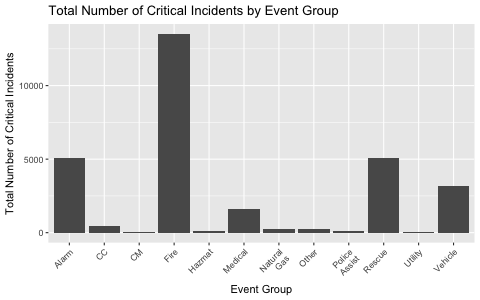
\includegraphics[width=\textwidth]{total_critical_incidents_by_event_group}
		\caption{The above figure shows the unequal distribution of critical incidents to various event types. Most critical incidents occur during an alarm, fire, rescue or vehicle event.
			\label{fig:critical-events}
		}
\end{wrapfigure}

After training the model on the training set, probabilities were assigned to observations in the test set. Observations with a probability of critical greater than 0.5 were classified as critical and all other observations were classified as non-critical. The confusion matrix of this classification is presented in Table~\ref{tab:lr-cm} and contains favourable results.

Table~\ref{tab:lr-stats} contains the calculated evaluation metrics for the associated confusion matrix. Accuracy of 92\% is acceptable for early attempts but this value is likely to be able to be increased with more fine tuning of the model. Note that by assigning Non-critical to every class you would receive an accuracy of 79\% due to the class imbalance. This is why Precision, Recall and F\textsubscript{1}-Score are also calculated as they depend on the presence of True Positives (correctly predicting the presence of the class attribute) and thus are well suited for class imbalances.

\begin{wraptable}[19]{l}{0.3\textwidth}
	\begin{subfigure}[h]{\textwidth}
		\centering
		\begin{tabular}{@{}cc cc@{}}
		\multicolumn{1}{c}{} &\multicolumn{1}{c}{} &\multicolumn{2}{c}{Predicted} \\ 
		\cmidrule(lr){3-4}
		\multicolumn{1}{c}{} & 
		\multicolumn{1}{c}{} & 
		\multicolumn{1}{c}{0} & 
		\multicolumn{1}{c}{1} \\ 
		\cline{2-4}
		\multirow[c]{2}{*}{\rotatebox[origin=tr]{90}{Actual}}
		& 0  & 19423 & 1175   \\[1.5ex]
		& 1  & 383   & 3717 \\ 
		\cline{2-4}
		% \caption{
		% 	Confusion Matrix of Logistic Regression classifier on FIRE incidents. 0 and 1 represent critical and non-critical incidents, respectively.
		% 	\label{tab:lr-cm}
		% }
		\end{tabular}
		\caption{
			Confusion Matrix
			\label{tab:lr-cm}
		}
	\end{subfigure}
	\begin{subfigure}[h]{\textwidth}
		\begin{tabular}{l r}\toprule
			Statistic & Value (\%) \\ \midrule
			Accuracy & 91.6 \\
			False-Negative Rate & 31.5 \\
			Precision & 90.6 \\
			Recall & 68.4 \\
			F\textsubscript{1}-Score & 77.9 \\ \bottomrule
		\end{tabular}
		\caption{Evaluation Metrics
			\label{tab:lr-stats}
		}
	\end{subfigure}
	\caption{A confusion matrix and corresponding evaluation metrics for Logistic Regression classifier on fire incidents.	0 and 1 represent non-critical and critical incidents, respectively}

\end{wraptable}

\subsection{Fire Class: Binary Class with Naive Bayes \& Random Forest}

In order to benchmark the performance of the Logistic Regression classifier the critical incidents were also predicted using Naive Bayes and Random Forest classifiers. The general formula and features presented above were used for all models with some minor adjustments where necessary: Naive Bayes and Random Forest can only handle categorical input features with Random Forest having an upper limit on factor levels. To meet these requirements some adjustments were required.

Each model, including Logistic Regression, was trained and tested on ten different random samples with the resulting evaluation metrics recorded. Only fire incidents were used: the training sets comprised 60\% of the fire incident subset with the test sets accounting for the remaining 40\%. Accuracy, Precision, Recall and the F\textsubscript{1}-Score are plotted for each iteration in Figure~\ref{fig:eval-3models} while the averages for the corresponding metrics, across the 10 iterations, is presented in Table~\ref{tab:3model-ave}.

\section{Model Evaluation}

Accuracy is the metric with the least variance between models and between iterations. This might partly be attributed to the class imbalance: a null model would achieve accuracy of 79\% by simply predicting every incident to be non-critical! That only leaves a 21\% margin for improvement. With this in mind the models improved the accuracy of the null model by between 11 and 14 percent which is a non-trivial amount.

The remaining three metrics; precision, recall, and F\textsubscript{1}-Score are dependent on the quantity of True Positives and thus would be 0 in the case of the null model. Precision is a percentage of predicted critical incidents that actually were (TP/TP+FP) whereas recall represents the percentage of critical incidents that were accurately identified (TP/TP+FN). F\textsubscript{1}-Score is the harmonic average of these two metrics (2TP/2TP+FP+FN). Using metrics with the quantity of True Positives as the numerator ensures that they are sensitive to models that aren't effective in the presence of a class imbalance: the null model would be 0 for all metrics!

\begin{wrapfigure}[25]{l}{0.4\textwidth}
	\centering
		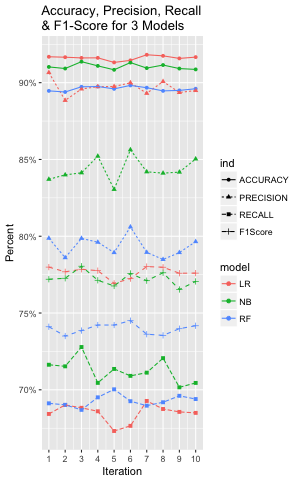
\includegraphics[width=\textwidth]{accuracy_precision_recall_3models}
		\caption{Accuracy, Precision, Recall \& F\textsubscript{1}-Score plotted for each iteration of the 3 models
			\label{fig:eval-3models}
		}
\end{wrapfigure}

Depending on a specific application a model may be trained to maximize a certain metric: perhaps some situations demand high recall, others high precision, and some still where a balance between the two is most desirable. Among the three models trained and tested in this project Linear Regression had the highest percentage of correctly predicted critical incidents (Precision). Conversely, however, it identified on average the lowest percentage of actual critical incidents (Recall), although in this case the average difference between the other models is significantly less. This relationship brings the F\textsubscript{1}-Score for the three models much closer together, especially between Linear Regression and Naive Bayes which alternate between maximizing precision and recall, respectively. 



\subsection{ANOVA}
A One-way Analysis of Variance was run on the ten Accuracy and F\textsubscript{1}-Score metrics produced from each model's test set predictions. The corresponding ANOVA tables are provided for Accuracy and F\textsubscript{1}-Score in Table~\ref{tab:anova-accuracy} and Table~\ref{tab:anova-F1}, respectively.

The p-value represents the probability that the averages for the corresponding metrics are from the same population and are both incredibly low for each metric tested. Thus it is safe to conclude, with 99\% confidence,

\begin{wraptable}{l}{0.6\textwidth}
	\begin{tabular}{l l l l l} \toprule
		Model & Accuracy & Precision & Recall & F\textsubscript{1}-Score \\ \midrule
		Logistic Regression & 91.61 & 89.68 & 68.49 & 77.66 \\
		Naive Bayes & 91.04 & 84.32 & 71.24 & 77.22 \\
		Random Forest & 89.60 & 79.35 & 69.27 & 73.97 \\
		\caption{Average evaluation metrics for the 3 models run in this project
			\label{tab:3model-ave}
		}
	\end{tabular}

\end{wraptable}

\noindent that the evaluation metrics were sampled from different populations and thus the choice of model will impact the resulting predictive performance. Not shown, however, are the associated coefficients and p-values for differences between the models F\textsubscript{1}-Score: perhaps as expected by the very close averages for F\textsubscript{1}-Score between Logistic Regression and Naive Bayes there is a much lower p-value for a difference between these two models. Although the difference is still significant, it is much less so with a p-value of 0.0152, which corresponds to the 95\% confidence level. This means there is strong evidence for a difference of F\textsubscript{1}-Scores between the three models, but much less of a difference between Naive Bayes and Logistic Regression.

\clearpage

\begin{wraptable}[13]{r}{0.6\textwidth}
	\begin{subfigure}[h]{\textwidth}
		\begin{tabular}{l l l l l l} \toprule
			& Df & Sum Sq & Mean Sq & F value & Pr($>$F) \\ \midrule
			model & 2 & 2.15e-03 & 1.07e-03 & 4.35.32 & $<$ 2.2e-16 \\
			Residulas 27 & 6.69e-05 & 2.48e-06 & & \\
		\end{tabular}
		\caption{
			Accuracy vs. Model
			\label{tab:anova-accuracy}
		}
	\end{subfigure}
	\begin{subfigure}[h]{\textwidth}
		\begin{tabular}{l l l l l l} \toprule
			& Df & Sum Sq & Mean Sq & F value & Pr($>$F) \\ \midrule
			model & 2 & 0.00814 & 0.00407 & 288.81 & $<$ 2.2e-16 \\
			Residulas 26 & 0.00038 & 0.00001 & & \\
		\end{tabular}
		\caption{
			F\textsubscript{1}-Score vs. Model
			\label{tab:anova-F1}
		}
	\end{subfigure}
	\caption{One-way ANOVA to test for differences in Accuracy and F\textsubscript{1}-Score between the three models.}

\end{wraptable}

\section{Conclusion}
A fire incident dataset was obtained from an open data catalogue, converted to tabular structure, and subjected to preparation followed by an exploratory data analysis. Trends and relationships between features were explored before a binary class attribute was assigned based on features available following an incident. Three predictive models were then used to predict the class attribute using a different set of features which would be available at the time of incident call. Each model was trained on 10 randomly selected training sets, comprising 60\% of a subset of the data, and then used to make predictions on the corresponding test set which accounted for the other 40\%. Four evaluation criteria were then selected; three due to their sensitivity to the imbalance that existed in the class attribute. Generally speaking Logistic Regression and Naive Bayes were the two most successful models, with the highest precision and recall respectively. As they alternated between highest performance on these two metrics the average between them, F\textsubscript{1}-Score, was much closer but still significant. In closing the models performed well and are likely suitable for implementation into a Computer Aided Dispatch system to provide fire services first responders with improved incident information at the time of call.

\section{References}
{\parindent0pt
\medskip Asgary, A., Naini, AS., \& Levy, J. (2012). Modeling the risk of structural fire incidents using a self-organizing map. Fire Safety Journal, 49, 1-9.doi:10.1016/j.firesaf.2011.12.007

\medskip Asgary, A., \& Sadeghi-Naini, A. (2013) Modeling number of firefighters responding to an incident using artificial neural networks. International Journal of Emergency Services, 2(2), 104-18.doi:10.1108/IJES-03-2012-0001

\medskip Asgary, A., Sadeghi-Naini, A., \& Levy, J. (2009). Intelligent Security Systems Engineering for Modeling Fire Critical Incidents: Towards Sustainable Security. Journal of Systems Science and Systems Engineering, 18(4), 477-488.doi:10.1007/s11518-009-5121-2

\medskip Asgary, A., Sadeghi-Naini, A., \& Kong, A. (2009). Modeling loss and no-loss fire incidents using artificial neural network: Case of Toronto. Science and Technology for Humanity, 159-163.doi:10.1109/TIC-STH.2009.5444513

% I don't have the below (polish?) Unicode. 
% Ceyhan, E., Ertŭgay, K., \& Düzgün, Ş. (2013). Exploratory and inferential methods for spatio-temporal analysis of residential fire clustering in urban areas. Fire Safety Journal, 58, 226-249.doi:10.1016/j.firesaf.2013.01.024
\medskip Ceyhan, E., Ert\v{u}gay, K., \& Düzgün, Ş. (2013). Exploratory and inferential methods for spatio-temporal analysis of residential fire clustering in urban areas. Fire Safety Journal, 58, 226-249.doi:10.1016/j.firesaf.2013.01.024

\medskip Asgary, A., Ghaffari, A., Levy, J. (2009). Spatial and temporal analyses of structural fire incidents and their causes: A case of Toronto, Canada. Fire Safety Journal, 45, 44-57.doi:10.1016/j.firesaf.2009.10.002

\medskip Sekizawa, A. (2012). Necessity of Fire Statistics and Analysis Using Fire Incident Database - Japanese Case -. Fire Science and Technology, 31(3), 67-75.doi:10.3210/fst.31.67

\medskip Bergen, G., Frattaroli, S., Ballesteros M.F., Ta, V.M., Beach, C., \& Gielen, A.C. (2008) J Community Health, 33, 103-109.doi:10.1007/s10900-007-9070-8

\medskip KrishnaVeni, C.V, \& Rani, T.S. (2011) On the Classification of Imbalanced Datasets. International Journal of Computer Science \& Technology. 145-148. Retrieved from http://ijcst.com/icaccbie11/sp1/krishnaveni.pdf

\medskip López, V., Fernandez, A., Garcia, S., Palade, V.,  \& Herrera, F. (2013) An Insight into Classification with Imbalanced Data: Empirical Results and Current Trends on Using Data Intrinsic Characteristics. Information Sciences, 250, 113-141.doi:10.1016/j.ins.2013.07.007

\medskip Mendenhall, W., Beaver, R., \& Beaver, B. (2013) Introduction to Probability and Statistics. Boston, MA: Brooks/Cole

\medskip Walmsley, P. (2007) XQuery. Sebastopol, CA: O’Reilly Media, Inc. 

\medskip Ripley, B.D., \& Hornik, K. (2001) Date-Time Classes. R News, 1(2), 8-11. Retrieved from http://cran.r-project.org/doc/Rnews/Rnews\_2001-2.pdf 

\medskip Bebee, D., (2012) New dispatch system helps fire department reduce response times: The Record. Retrieved from http://www.oafc.on.ca/article/new-dispatch-system-helps-fire-department-reduce-response-times

\medskip G. Casella, S. Fienberg, I. Olkin, (2013). An introduction to statistical learning: with applications in R. New York, NY: Springer Science+Business Media
Fire Services Incident Data: City of Toronto Open Data Catalogue (2018). Retrieved from https://www.toronto.ca/city-government/data-research-maps/open-data/open-data-catalogue/\\*\#e3d443bb-2593-2615-4972-20e24c0ab876 under the Open Data License: https://www.toronto.ca/city-government/data-research-maps/open-data/open-data-licence/

}
\end{document}

